
%(BEGIN_QUESTION)
% Copyright 2013, Tony R. Kuphaldt, released under the Creative Commons Attribution License (v 1.0)
% This means you may do almost anything with this work of mine, so long as you give me proper credit

Assess the status of this relay circuit, given the following (simultaneous) switch actuation statuses:

\begin{itemize}
\item{} Switch A = {\it pressed}
\item{} Switch B = {\it unpressed}
\item{} Switch C = {\it pressed}
\end{itemize}

$$\includegraphics[width=15.5cm]{i03055x01.eps}$$

Now, check the appropriate cells in this table indicating whether each of the specified components is {\it energized} (powered) or {\it de-energized} (unpowered):

% No blank lines allowed between lines of an \halign structure!
% I use comments (%) instead, so that TeX doesn't choke.

$$\vbox{\offinterlineskip
\halign{\strut
\vrule \quad\hfil # \ \hfil & 
\vrule \quad\hfil # \ \hfil & 
\vrule \quad\hfil # \ \hfil \vrule \cr
\noalign{\hrule}
%
% First row
{\bf Component} & {\bf Energized} & {\bf De-energized} \cr
%
\noalign{\hrule}
%
% Another row
Red lamp &  &  \cr
%
\noalign{\hrule}
%
% Another row
Green lamp &  &  \cr
%
\noalign{\hrule}
%
% Another row
CR1 coil &  &  \cr
%
\noalign{\hrule}
} % End of \halign 
}$$ % End of \vbox

\underbar{file i03055}
%(END_QUESTION)





%(BEGIN_ANSWER)

% No blank lines allowed between lines of an \halign structure!
% I use comments (%) instead, so that TeX doesn't choke.

$$\vbox{\offinterlineskip
\halign{\strut
\vrule \quad\hfil # \ \hfil & 
\vrule \quad\hfil # \ \hfil & 
\vrule \quad\hfil # \ \hfil \vrule \cr
\noalign{\hrule}
%
% First row
{\bf Component} & {\bf Energized} & {\bf De-energized} \cr
%
\noalign{\hrule}
%
% Another row
Red lamp & $\surd$ &  \cr
%
\noalign{\hrule}
%
% Another row
Green lamp &  & $\surd$ \cr
%
\noalign{\hrule}
%
% Another row
CR1 coil & $\surd$ &  \cr
%
\noalign{\hrule}
} % End of \halign 
}$$ % End of \vbox


%(END_ANSWER)





%(BEGIN_NOTES)

{\bf This question is intended for exams only and not worksheets!}.

%(END_NOTES)

